\documentclass[../Head/Main.tex]{subfiles}
\begin{document}
	\begin{tikzpicture}
		\node[anchor=south west, inner sep=0] (image) at (0,0) {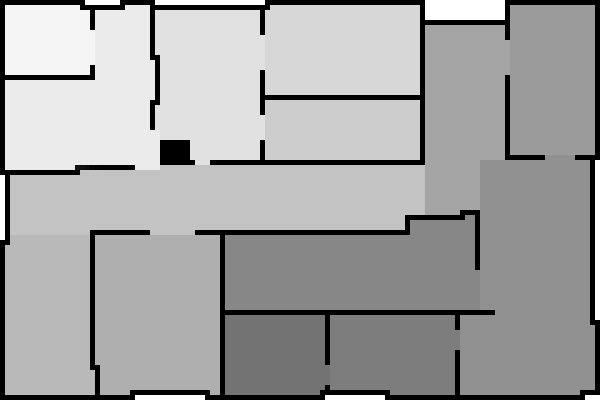
\includegraphics[width=\textwidth]{map_medium}};
		%\node[align=center, black, font={\large\bfseries}] at (1,7.7) {Room 1};
		%\node[align=center, black, font={\large\bfseries}] at (1.75,6) {Room 2};
		%\node[align=center, black, font={\large\bfseries}] at (4.5,6.75) {Room 3};
		%\node[align=center, black, font={\large\bfseries}] at (7.25,7.5) {Room 4};
		%\node[align=center, black, font={\large\bfseries}] at (7.25,5.75) {Room 5};
		%\node[align=center, black, font={\large\bfseries}] at (5,4.25) {Room 6};
		%\node[align=center, black, font={\large\bfseries}] at (1,2) {Room 7};
		%\node[align=center, black, font={\large\bfseries}] at (3.3,2) {Room 8};
		%\node[align=center, black, font={\large\bfseries}] at (9.9,6.25) {Room 9};
		%\node[align=center, black, font={\large\bfseries}] at (11.75,6.75) {Room 10};
		%\node[align=center, black, font={\large\bfseries}] at (11.5,2.5) {Room 11};
		%\node[align=center, black, font={\large\bfseries}] at (7.25,2.75) {Room 12};
		%\node[align=center, black, font={\large\bfseries}] at (8.25,1) {Room 13};
		%\node[align=center, black, font={\large\bfseries}] at (5.8,1) {Room 14};
	\end{tikzpicture}
\end{document}